\documentclass[a4paper,11pt]{article}
\usepackage[left=2.5cm, right=2.5cm, top=1.5cm, bottom=1.5cm]{geometry}
\usepackage{graphicx}
\usepackage{amssymb}
\usepackage{amsmath}
\usepackage[procnames]{listings}
\usepackage{xcolor}
\usepackage{hyperref}
\usepackage{cleveref}

\hypersetup{ %color attributes of citation, link, etc.
    colorlinks=true,
    linkcolor=blue,
    filecolor=gray,
    urlcolor=blue,
    citecolor=blue,
}

\setlength{\parindent}{0pt}

\newcommand\Item[1][]{%
  \ifx\relax#1\relax  \item \else \item[#1] \fi
  \abovedisplayskip=0pt\abovedisplayshortskip=0pt~\vspace*{-\baselineskip}}

%'codify' text for snippets
\definecolor{codegray}{gray}{1}
\newcommand{\code}[1]{\colorbox{codegray}{\texttt{#1}}}

\graphicspath{ {images/} }
           
\begin{document}
\title{\LARGE{\textbf{A Review of Mechatronic Chordophone Pickers \& Dampers}}}
\author{Niels Clayton : 300437590}
\date{}
\maketitle
\hrule

\section{Overview}

The field of mechatronic instruments aims to expand upon the human experiences of composing and performing music. Mechatronic instruments have the ability assist and enhance music playing, as well as producing new types of music that a human would find difficult or not be capable of replicating \cite{Ogata2017}. The mechatronic chordophone provides a fast and precise method of producing music with stringed instruments \cite{YepezPlacencia2020}. Below in \Cref{F:basic_design}, the base components of a mechatronic chordophone are outlined. This review we will outline different picking and damping mechanisms, and will look to identify their advantages and limitations. 

\begin{figure}[h!]
  \begin{center}
    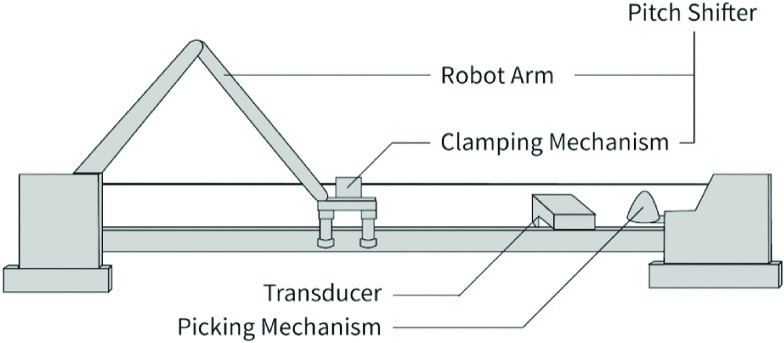
\includegraphics[width=0.8\textwidth]{chordophone_design.jpg}
    \caption{Overview of common mechatronic chordophone construction \cite{YepezPlacencia2020}}
    \label{F:basic_design}
  \end{center}
\end{figure}


\section{Review of Literature}
\subsection{Mechatronic Picking Mechanisms}

 Most common mechatronic picking mechanisms can be categorised by the actuators they use for picking. Solenoids actuator designs tend to provide a linear motion of the pick back and forth over the string, while stepper motors have a rotary motion with large numbers of picks located in a central hub. 

\subsubsection{Solenoid Actuated Picking Mechanisms}

Solenoid actuator based picking mechanisms present a very simple to implement and cost effective design, as solenoids are inexpensive and do not require any driving circuitry other than a simple MOSFET \cite{Kapur2011ACO}. Existing picking designs such as the Poly-tangent Automatic (multi-)Monochord (PAM) \cite{Rogers} are based on using two solenoid actuators in a push-pull configuration, moving the pick back and forth across the string. This picking system was recreated at Wellington University Victoria, and demonstrated a picking speed of 20 nps (notes per second).

Due to the back and forth motion of the pick using this method, it has been suggested that this design allows for a more accurate recreation of actual human strumming \cite{Placencia2020}. However it has also be demonstrated that small differences in the two solenoids will lead to very large acoustic differences between the backwards and forwards stroke of the pick \cite{Kapur2011ACO}. It has also been said that the back and forth motion of this pick will constrain the picking angle to being vertical, as any other picking angle will have drastically different forward and backward interactions \cite{Carnegie2020}. 

\subsubsection{Stepper Motor Actuated Picking Mechanisms}

Stepper motor actuated picking mechanisms tend to come in the form of a 'pick-wheel', with multiple picks mounted to a single motor. The design of these pick-wheels allows for varying pick attack angles, as well as varying the numbers of picks per full rotation of the motor \cite{YepezPlacencia2020, Carnegie2020}. According to these sources, a stepper motor based picker is capable of achieving picking speeds of 25 nps.

A well developed example of this style of picking mechanism can be found in the 'MechBase' \cite{McVay2015}, which consists of a pick-wheel with five picks attached. The picking mechanism from 'MechBase' also allows for adjustment of loudness and timbre, by adjusting the position of the pick-wheel using a servo driven pivot \cite{Carnegie2020}. This allows the 'MechBase' to produce a wider range of picking effects, and more accurately recreate human playing. 

This style of actuator has also had a mechanism designed that allows for dynamic adjustment of the picking angle, using a second stepper motor and a worm gear to hold each of the picks \cite{Carnegie2020}. However, This method of adjusting the pick angle doubles the electromagnetic noised generated by the motors, and currently does not allow for changes of the mounting height to adjust loudness and timbre. 

\subsubsection{Novel Picking Mechanisms}

There also exist a selection of more novel picking mechanisms the allow for the generation of of a wide array of different sounds. One such mechanism is found Robotically Augmented Electric Guitar \cite{Ogata2017}, which uses an array of actuatable hammers built into an electric guitar. This design looks to enhance the playing of the instrument by adding fast rhythmic patterns alongside the normal playing. Another novel actuation and picking method is presented by Steven Kemper, in which DC vibration motors are used to very quickly agitate the string, producing a mechatronic 'tremolo' effect \cite{Kemper2020}.


\subsection{Mechatronic Damping Mechanisms}

The ability stop or decrease the vibration of an instruments strings allows for the articulation of specific notes, and is a pivotal components of a mechatronic chordophone \cite{YepezPlacencia2020}. The literature reviewed presented two different mechanisms to actuate this damping, either using a solenoid such as in the LEMUR 'GuitarBot' \cite{Singer2003}, or a servo motor such as in the 'MechBase' \cite{McVay2015}. 
Both of these damping mechanisms work on the same basic principle, and remove energy from the vibrating string by contacting it with a foam, soft plastic or polymer. Servo based damping mechanisms have an advantage in that they are able to dynamically adjust the damping by varying the force applied to to string.


\section{Discussion}

% say some shit about how there is a wide variety of mechanisms they all have their specific uses depending on what you are wanting to achieve with your instrument. Also talk about how there seems to be a gap in the development of novel damping mechanisms.


\newpage
\bibliographystyle{ieeetr}
\bibliography{references}
\end{document}